\section{Pilot Application}

In this network environment, we focus on consumer-facing applications, as shown in Figure~\ref{fig:continuum}. 
Mobile physical activity monitoring applications
(fitness tracker) with location-based content push.

For our use case, focus on a \textbf{simple ecosystem of composable services rather than a single siloed application.}

Our pilot application:  \textbf{NDNEx} (NDN-Exercise) and a user-facing \textbf{Identity Manager}.  Supporting physical activity is both a critical part of building healthy communities and a key retail market. 

Our objective is not only an application.

It is to act as an example of interoperating components of an Open mHealth ecosystem.

This places additional requirements on the design.

See Deborah's TEDMED talk: 
\url{https://www.youtube.com/watch?feature=player_embedded&v=lAEhSGYEHWU}


\begin{figure*}
\begin{center}
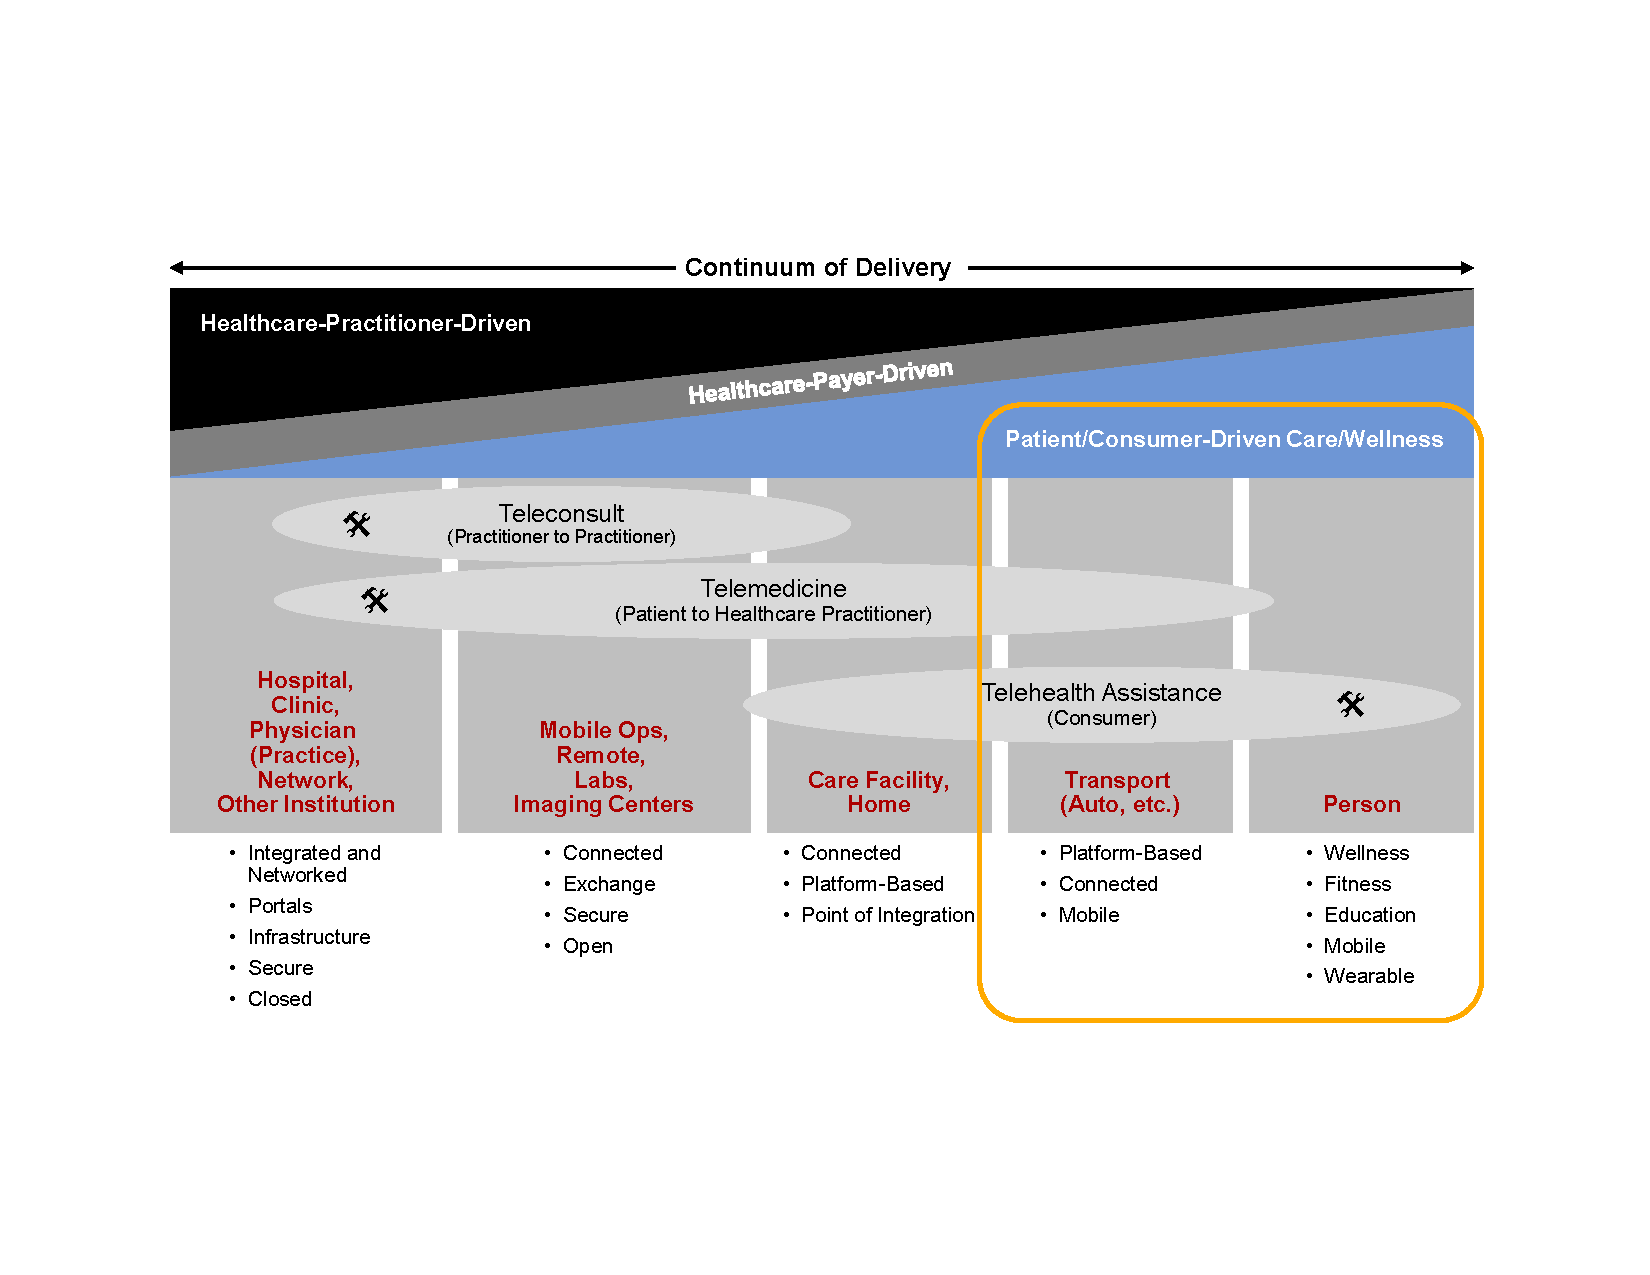
\includegraphics[width=.8\textwidth]{figures/continuum}
\caption{{Focus of Open mHealth network environment shown in yellow box. Figure from Gartner, 2013.  }}
% A Framework for Understanding Telehealth, Telemedicine and Other Remote Healthcare Delivery Solutions
% need to redraw before release
\label{fig:continuum}
\end{center}
\end{figure*}


NDNEx is a non-proprietary ecosystem for consumer physical activity data. 

Start with end-user mobile+web application that captures and reports walking, jogging, and running activity.

Calculate and report activity metrics based on GPS and accelerometer data  both automatically and self-identified rounds of exercise.  

Ad-hoc and formal groups or teams. 

Capable of location-based content push during the exercise, which can be used for health, entertainment, local, and team-related content. 

Commercial parallels:  Nike+, Fitbit, Endomondo (see Figure~\ref{fig:endomondo}), etc. 

\begin{figure}
\begin{center}
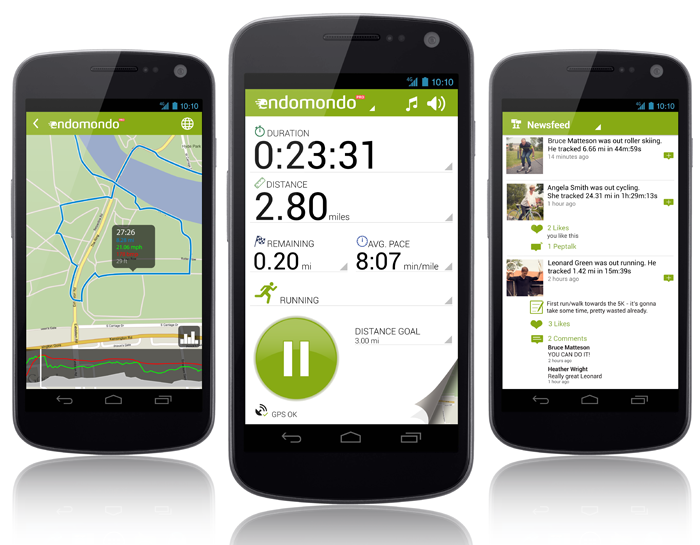
\includegraphics[width=.6\textwidth]{figures/endomondo}
\caption{Endomondo commercial fitness tracker. \protect\url{https://www.endomondo.com/}}
\label{fig:endomondo}
\end{center}
\end{figure}


Envisioned as an open-data ecosystem, with different service providers at different stages in the processing chain, rather than a siloed application.

Work that we can leverage (see related work above): 

Open mHealth Toolset  including Ohmage reference platform and the Lifestreams concept. 

Past CENS/UCLA participatory sensing research in activity classification,self-surveillance privacy, mobile phone based data collection.

REMAPs funded collaborations on Urban Trails and technology for Parks with California State Parks, the Western National Parks Association, National Park Service, and the City of Los Angeles. 

\begin{figure}
\begin{center}
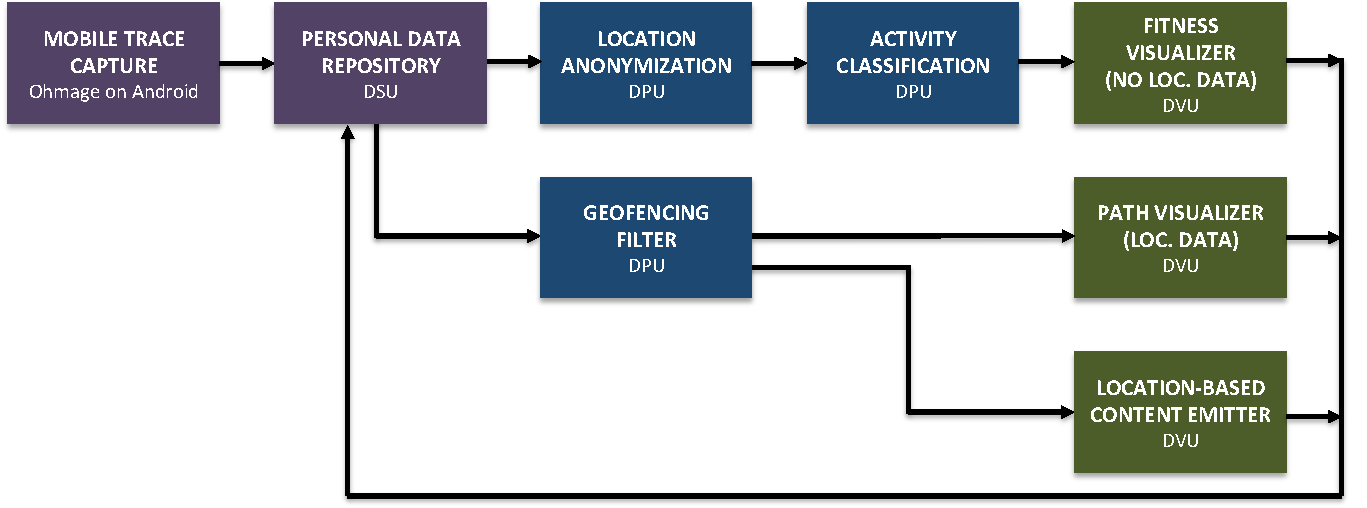
\includegraphics[width=1\textwidth]{figures/ConceptualBlock}
\caption{Conceptual block diagram showing data flow.}
\label{fig:ConceptualBlock}
\end{center}
\end{figure}



\subsection{Application Requirements}

For this application in particular, NDN provides much more relevant functionality at the network layer than IP.  
So solutions in NDN have much more direct impact on the scalability, security, and ease of development; we need not build up additional layers on IP to get near the app challenges.

Cite hourglass figure 

\begin{itemize}
\item Namespace / schema design
\item Repository / storage design
\item Service composability
\item Authentication / identity assurance
\item Data provenance
\item Access auditing
\item Mobile publishing
\item Legal requirements for success
\end{itemize}

The Open mHealth team envisions that the Internet will interconnect 1)
data capture, 2) secure storage, 3) modeling and analytics, and 4) user
interface components to create a modular, layered sense-making framework.  
%% Repeated from above.

Adaptation of Open mHealth REST-based communication model to a data dissemination approach inspired by NDN.

\subsubsection{Naming} 
\begin{itemize}
\item \textbf{Data format namespace design} comes directly from Open mHealth developer documentation. 
\item \textbf{Application architecture} consistent with the pieces above and from previous participatory sensing projects. (e.g., Mun et al, 2009)
\item What schema? Initially, try direct mapping of Open mHealth schema
\item Borrow ideas from Named Function Networking concept for distributed processing
\item Translate existing REST-based approach or do pure NDN? 
\item Represent raw time-location data (GPS, accelerometer) from mobiles. 
\item Support successive rounds of processing that, for example:  
    \begin{itemize}
    \item Generate classified activity data that follows the Physical Activity JSON schema and perhaps other related schemas.  (This happens at client-side in Ohmage Mobility but could happen at a DPU.)	
    \item Identify / segment ``bouts”''of physical activity or exercise. 
    \item Add features to a bout from DPUs to the existing store. 
    \end{itemize}
\item Consumers should be able to access raw and processed data for a certain time period.
\item Consumers should be able to efficiently read data sequentially. 
\end{itemize}

\subsubsection{Trust and security}

Fit NDN architectural mechanisms into security requirements
\begin{itemize}
\item \textbf{Identity and trust management} scenario comes from our proposed application use case.  (Recall:  Not just an app, an example of interoperating components in an ecosystem.)
\item Provide granular access control over various components of the data namespace – in particular, raw location data. 
\item Replacing Oauth2 for distributed processing is critical
\item Data encryption requirements
\item Name privacy issues
\item Follow passive key publication approach (rather than active) if possible. 
\end{itemize}
Can / should we support different identities relative each part of the system: collection, processing, and visualization?
Collection: User may publish data to serve multiple applications, but doesn’t want them to be able to conspire / correlate that they are the same user.
Processing:  Design should provide the minimum possible information to the processing components about user identity. 
Visualization: Visible face of “the app” to the user. 

\subsubsection{Storage in the network}
\begin{itemize}
\item Interaction of personal and shared stores
\item Data filtering at the repo?
\item New legal / economic relationship between the players
\end{itemize}
